\documentclass[a4paper]{article}

\usepackage[T1]{fontenc}
\usepackage{textcomp}
\usepackage{mathtools,amssymb,amsthm}
\usepackage[hmargin=1in,vmargin=1in]{geometry}
\usepackage{graphicx,cancel}
\usepackage[math-style=TeX]{unicode-math}
% \usepackage[lite,subscriptcorrection,nofontinfo]{mtpro2}
\usepackage{fontspec}
\usepackage[colorlinks=true,allcolors=blue]{hyperref}

\defaultfontfeatures{Ligatures=TeX,Numbers=OldStyle}
\setmainfont{Palatino Linotype}
\setmathfont{TeX Gyre Pagella Math}
%\usepackage[integrals]{wasysym}
\frenchspacing

\newcommand*{\parasp}{\setlength{\parskip}{10pt plus 2pt minus 3pt}}
\newcommand*{\noparasp}{\setlength{\parskip}{0pt plus 1pt}}
\newcommand*{\setparasp}[1]{\setlength{\parskip}{#1}}
\newcommand*{\pskip}{\vskip 10pt plus 2pt minus 3pt}
\newcommand\LEFTRIGHT[3]{\left#1 #3 \right#2}
\newcommand*{\paren}[1]{\LEFTRIGHT(){#1}}
\newcommand*{\brkt}[1]{\LEFTRIGHT[]{#1}}
\newcommand*{\unit}[1]{\,\mathrm{#1}}
\newcommand*{\DeclareUnit}[2]{\newcommand*{#1}{\unit{#2}}}
\DeclareUnit{\cm}{cm}
% \renewcommand*{\m}{\unit{m}}
\DeclareUnit{\m}{m}
\DeclareUnit{\kg}{kg}
\DeclareUnit{\s}{s}
\newcommand*{\R}{\mathbb{R}}
\newcommand*{\Rp}{(0,+\infty)}
\newcommand*{\Rm}{(-\infty,0)}
\newcommand*{\deduce}{\mathrel{\Downarrow}}
\newcommand*{\abs}[1]{\left\lvert #1 \right\rvert}
\newcommand*{\reason}[1]{\langle \, \text{#1} \, \rangle}

\newcounter{ListCounter}
\newenvironment{enumerate*}%
{\begin{list}%
        {\arabic{ListCounter}.}%
        {\usecounter{ListCounter}%
            \setlength{\topsep}{1.5pt}%
            \setlength{\itemsep}{1.5pt} } }%
    {\end{list}}

\DeclareMathOperator{\arccosh}{arccosh}
\DeclareMathOperator{\gammaf}{\Gamma}
\DeclareMathOperator{\var}{var}
\DeclareMathOperator{\Ber}{Bernoulli}
\DeclareMathOperator{\Cov}{Cov}
\DeclareMathOperator{\E}{E}
%\newcommand*{\diff}{\mathop{}\!d}
\newcommand*{\diff}{\mathop{}\!\mathit{d}}
%\newcommand*{\diff}{\mathop{}\!\mathrm{d}}
\newcommand*{\dx}{\diff x}
\newcommand*{\dy}{\diff y}
\newcommand*{\dz}{\diff z}
\newcommand*{\dt}{\diff t}
\newcommand*{\du}{\diff u}
\newcommand*{\dv}{\diff v}
\newcommand*{\dtheta}{\diff \theta}
\newcommand*{\ddx}{\frac{\diff}{\dx}}
\newcommand*{\fwdf}{\mathop{}\!\Delta}
\newcommand*{\dydx}{\frac\dy\dx}
\newcommand*{\pdpdx}{\frac\partial{\partial x}}
\newcommand*{\pdpdy}{\frac\partial{\partial y}}
\newcommand*{\pdpdz}{\frac\partial{\partial z}}
\newcommand*{\pdpdu}{\frac\partial{\partial u}}
\newcommand*{\pdpdv}{\frac\partial{\partial v}}
\newcommand*{\pdpdt}{\frac\partial{\partial t}}
\newcommand*{\pdzpdx}{\frac{\partial z}{\partial x}}
\newcommand*{\pdzpdy}{\frac{\partial z}{\partial y}}
\newcommand*{\pdzpdt}{\frac{\partial z}{\partial t}}
\newcommand*{\pdxpdt}{\frac{\partial x}{\partial t}}
\newcommand*{\pdypdt}{\frac{\partial y}{\partial t}}

\AtBeginDocument{%
	\renewcommand{\perp}{\mathrel{\bot}}
	\let\leq\leqslant
	\let\le\leq
        \let\geq\geqslant
        \let\ge\geq}

\newcommand*{\Prb}[1]{\section*{Problem #1}}
\newcommand{\Q}[1]{\textbf{Question:} #1}
\newcommand*{\A}[1]{\textbf{Answer:} #1}
\newcommand{\Prblm}[3]{\Prb{#1} \Q{#2} \\[6pt] \A{#3}}


\usepackage{ellipsis, mathtools}

\renewcommand{\baselinestretch}{1.15}

\begin{document}
    
    \Prblm{3}
    {\par\parasp\noindent
    \textbf{For the brave:} The following model of a biochemical ``switch''
    comes from the (very pleasant) text of Strogatz, \emph{Nonlinear Dynamics
    and Chaos}. Let $ G(t) $ denote a concentration of a certain gene product,
    where the gene is switched ``on'' or ``of{}f'' depending on the presence of
    a chemical signal. The production of $ G $ is inf{}luenced both by the
    chemical signal and by \emph{autocatalysis} (a feedback mechanism) and decay
    (a natural degradation). After simplification, the behavior of $ G $
    follows:
        \[ \frac{dG}{dt} = a - bG - \frac{G}{1+G^2}, \]
    where $ a $ and $ b $ are positive constants and $ G(t) \ge 0 $.
    
    The number and types of equilibria depend on the values of $ a $ and $ b $.
    Unfortunately, solving for them analytically (that is, finding exact values)
    is \dots\ challenging. Without determining exactly where the equilibria are,
    what can you say about them?}
    {\begin{table}[h]
        \begin{tabular}{lcl}
                & a. & For some values of $ a $ and $ b $, there are no
                equilibria. \\
            \checkmark
                & b. & There is always at least one equilibrium. \\
            \checkmark
                & c. & \parbox[t]{5in}{\setlength{\baselineskip}{1em} There are
                    at most three equilibria. When there are three, then two are
                    stable and one is unstable.} \\[1em]
                & d. & All equilibria are stable. \\
                & e. & All equilibria are unstable. \\
        \end{tabular}
    \end{table}}
    
    When $ G=0 $, $ {dG}/{dt} = a > 0 $. As $ G $ goes to positive
    infinitely, $ {G}/{(1+G^2)} $ approaches zero, $ bG $ goes to positive
    infinity and $ a $ is always a constant; thus the leading term of $
    {dG}/{dt} $ is $ -bG $. Hence $ {dG}/{dt} $ approaches negative
    infinity as $ G $ approaches positive infinity. By intermediate value
    theorem (IVT), $ {dG}/{dt} $ must has a zero on $ \Rp $. That is to say,
    there is always an equilibrium. Therefore, a.\ is incorrect and b.\ is
    correct.
    
    Now we know that at least one equilibrium exists and we shall then
    investigate the number of equilibria and the stableness of them. Let $
    \dot{G} $ denote $ {dG}/{dt} $, as often seen in physics context; however,
    for the convenience of this problem, we shall view $ \dot{G} $ as a function
    of $ G $, but not of $ t $. Therefore, when $ G $ is an equilibrium, $
    \dot{G} $ is zero and the sign of $ {d\dot{G}}/{dG} $ can tell whether $ G $
    is stable or unstable:
        \begin{align*}
            \frac{d\dot{G}}{dG} &= -b - \frac{1-G^2}{(1+G^2)^2} \\
                &= -b + \frac{1}{1+G^2} - \frac{2}{(1+G^2)^2} \\
            \shortintertext{and let $ X $ denote $ \dfrac1{1+G^2} $,
                then}
            \frac{d\dot{G}}{dG} &= -2X^2 + X - b.
        \end{align*}
    We can view this as a quadratic function of $ X $, whose domain is $ (0,1] $
    as a result of $ G \ge 0 $. The discriminant $ \Delta = 1 - 8b $ implies
    that $ {d\dot{G}}/{dG} $ is always negative when $ b > {1}/{8} $. In
    this situation, there is only one equilibrium and it's also stable.
    Therefore, e.\ is incorrect since we find one stable equilibrium. \pagebreak
        
    We can even make a stronger argument. When ${ b = {1}/{8} }$\,,\, ${
    {d\dot{G}}/{dG} }$ is zero only at $ X = {1}/{4} $. $ \dot{G} $ is
    still monotonically decreasing on $ \Rp $. This means there is still a unique
    stable equilibrium on $ \Rp{} $ even when $ b = {1}/{8} $.
    
    When $ 0 < b < {1}/{8} $\,,\, $ {d\dot{G}}/{dG} $ has two zeros at
        \[  X = \frac{-1 \pm \sqrt{1-8b}}{-4} = \frac{1}{4} \, (1 \mp
        \sqrt{1-8b}), \]
    and let $ X_1 $ and $ X_2 $ denote them respectively. $ 0 < b < {1}/{8} $
    implies $ 0 < \sqrt{1-8b} < 1 $, hence
        \[ 0 < X_1 < \frac{1}{4} < X_2 < \frac{1}{2}. \]
    By substituting back $ X_1 $ with $ \dfrac1{1+G_1^2} $ and $ X_2 $ with $
    \dfrac1{1+G_2^2} $, we get
        \[ 0 < \frac{1}{1+G_1^2} < \frac{1}{4} < \frac{1}{1+G_2^2} <
        \frac{1}{2}. \]
    From this, we can derive that
        \[ 1 < G_2 < \sqrt{3} < G_1 \]
    and that $ d\dot{G}/dG $ is negative for $ G \in (0,G_2) \cup
    (G_1,+\infty) $ and positive for $ G \in (G_2,G_1) $.
    
    For any $ b \in (0,1/8) $\,,\, there always exists a positive $ a = \sqrt{3}
    \, (b + 1/4) $ such that the equation $ {\dot{G} = a - bG - G/(1+G^2) = 0} $
    is satisfied at $ {G = \sqrt{3}} $. At this time, $ d\dot{G}/G $ is positive
    and this means there's an unstable equilibrium for some $ a $ and $ b $.
    Therefore, d.\ is incorrect since we find an unstable equilibrium.
    
    All we left is the choice c., which is a little bit trickier. I'll achieve
    this by using the following two propositions, which both assume $ 0 < b <
    1/8 $.
    
    {\raggedright
        \textbf{Proposition 1.} If there is no equilibrium between $ G_2 $ and $
        G_1 $, there are at most two equilibria.
            
        \textbf{Proposition 2.} If there is an equilibrium between $ G_2 $ and $
        G_1 $, then this is an unstable equilibrium and there are exactly two
        stable equilibria on $ (0,G_2) $ and $ (G_1,+\infty) $. }
    
    We've already shown that there is a unique stable equilibrium when $ b \ge
    1/8 $. The
    \href{http://mathworld.wolfram.com/TrichotomyLaw.html}{trichotomy law}
    (applied to $ b $ and $ 1/8 $) combined with proposition 1.\ and 2.\
    guarantees that there are at most three equilibria and when there are
    three, then two are stable and one is unstable. What we should do now is to
    justify these two propositions.
    
    The sign of $ d\dot{G}/dG $ indicates $ \dot{G} $ is strictly decreasing on
    $ [0,G_2] \cup [G_1,+\infty) $ and increasing on $ [G_2,G_1] $; therefore, $
    \dot{G}\,\vert_{G_2} $ is the absolute minimum on $ [0,G_1] $\,,\, $
    \dot{G}\,\vert_{G_1} $ is the absolute maximum on $ [G_2,+\infty) $\,,\, and
    $ \dot{G}\,\vert_{G_1} > \dot{G}\,\vert_{G_2} $.
    
    To justify proposition 1., the trichotomy law comes into play again. When
    evaluated at $ G=G_2 $,
         \[ \dot{G}\,\vert_{G_2} < 0 \quad \text{or} \quad \dot{G}\,\vert_{G_2}
         = 0 \quad \text{or} \quad \dot{G}\,\vert_{G_2} > 0, \]
    exclusively. When $ \dot{G}\,\vert_{G_1} > \dot{G}\,\vert_{G_2} > 0 $,
        \[ \dot{G}\,\vert_{G} \ge \dot{G}\,\vert_{G_2} > 0 \quad \text{for } G
        \in [0,G_1]\,, \]
     hence $ \dot{G} $ has no zero on $ [0,G_1] $ and exactly one zero on $
     (G_1,+\infty) $. When $ \dot{G}\,\vert_{G_1} > \dot{G}\,\vert_{G_2} = 0 $,
         \[ \dot{G}\,\vert_{G} > \dot{G}\,\vert_{G_2} = 0  \quad \text{for } G
         \in [0,G_1]\setminus\{G_2\}, \]
     hence $ \dot{G} $ has exactly two zeros at $ G=G_2 $ and on $ (G_1,+\infty)
     $. When $ \dot{G}\,\vert_{G_2} < 0 $, $ \dot{G}\,\vert_{G_1} \le 0 $ since there will be a zero on $ (G_2,G_1) $  if $ \dot{G}\,\vert_{G_1} > 0 $, which contradicts our assumption that there is no equilibrium on $ (G_2,G_1) $. Thus, $ \dot{G} $ has a zero on $ (0,G_2) $ and an optional zero at $ G=G_1 $ if $ \dot{G}\,\vert_{G_1} = 0 $. Therefore, proposition 1.\ is true.
     
     To justify proposition 2., the equilibrium between $ G_2 $ and $ G_1 $ must be unstable since $ d\dot{G}/G $ is positive on  $ (G_2,G_1) $. Let $ G_{\rm eq} $ denote this equilibrium, then
         \[ \dot{G}\,\vert_{G_1} > \dot{G}\,\vert_{G_{\rm eq}} = 0 >
         \dot{G}\,\vert_{G_2}. \]
     This means there are exactly two stable equilibrium on $ (0,G_2) $ and $ (G_1,+\infty) $. Therefore, proposition 2.\ is true.
    
    Therefore, c.\ is correct.
    
    \begin{figure}[h]
        \centering
        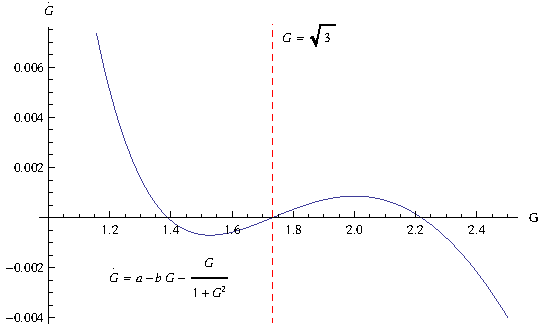
\includegraphics[width=0.7\linewidth]{hw20_challenge_fig1}
        \caption{$ \dot{G} $ with $ b = 0.12 < 0.125 $ and $ a = \sqrt{3}
            \, (b + 1/4) $}
        \label{fig:hw20_challenge_fig1}
    \end{figure}

    \begin{figure}[h]
        \centering
        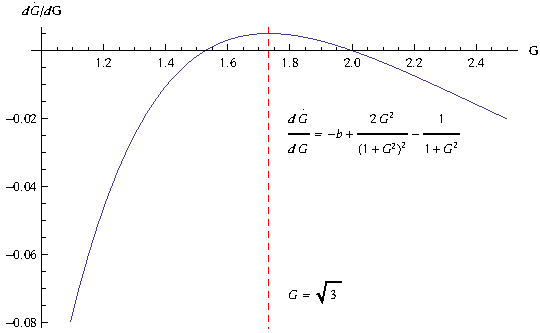
\includegraphics[width=0.7\linewidth]{hw20_challenge_fig2}
        \caption{$ \dfrac{d\dot{G}}{dG} $ with $ b = 0.12 < 0.125 $}
        \label{fig:hw20_challenge_fig2}
    \end{figure}
    
\end{document}